% BANZA Whitepaper v1.0 — PT edition. Generated from content/pt.json (single source).
\PassOptionsToPackage{table}{xcolor}

%% 2-column papers and preprints
\documentclass[journal abbreviation, manuscript]{copernicus}
\PassOptionsToPackage{english}{babel}
%\documentclass{copernicus}
\usepackage{textcomp}
\usepackage{listings}
\usepackage{savesym}
\usepackage{amsmath}
\savesymbol{unit}
\usepackage{float}
\usepackage{multicol}
\usepackage{siunitx}
\usepackage{todonotes}
\newcounter{todocounter}
\newcommand{\todonum}[2][]{\stepcounter{todocounter}\todo[#1]{\thetodocounter: #2}}
\usepackage{cancel}
% (integration) [table]{xcolor} is passed via \PassOptionsToPackage before the class — see line 1
\usepackage{colortbl}        % for coloring cells, rows, columns
\usepackage{booktabs}        % for nicer horizontal lines (\toprule, etc.)
%\title{BANZA: An Open Protocol for Financial Interoperability}
%\author{Fidel R. Monteiro \and Jesus R. Monteiro}
%\date{1 de agosto de 2026}
%\usepackage[portuguese]{babel}
\renewcommand{\abstractname}{Abstract}
\newcommand{\blfootnote}[1]{%
  \begingroup
  \renewcommand{\thefootnote}{}%
  \footnotetext{#1}%
  \addtocounter{footnote}{-1}%
  \endgroup
}
\makeatletter
\def\@@and{and}
% (EN) shared cls carries a PT-localised manuscript correspondence label; restore EN:
\usepackage{etoolbox}
\patchcmd{\@@maketitlemanuscript}{Correspondência:}{Correspondence:}{}{}
\renewcommand\Authand{ and }
\makeatother
%\emergencystretch=2em
% (integration) tighten the space reserved around in-text [H] figures so the approved 12-page
% composition packs as in the target edition (figures unchanged; only the float separation shrinks).
\setlength{\textfloatsep}{5pt plus 2pt minus 1pt}
\setlength{\intextsep}{5pt plus 2pt minus 1pt}
\setlength{\floatsep}{5pt plus 2pt minus 1pt}
% tighten displayed-equation spacing a touch so §2 (eqs 2--4 + Figure 2) packs onto one page as in the target
\setlength{\abovedisplayskip}{5pt plus 2pt minus 2pt}
\setlength{\belowdisplayskip}{5pt plus 2pt minus 2pt}
\setlength{\abovedisplayshortskip}{3pt plus 2pt}
\setlength{\belowdisplayshortskip}{4pt plus 2pt minus 2pt}
% (integration) recover the per-page line density of the target pdfLaTeX build under tectonic/XeTeX,
% whose OpenType Latin Modern metrics break a little looser; restores the approved 12-page pagination.
\addtolength{\textheight}{42pt}


\begin{document}
\selectlanguage{english}
% (integration) ini-based babel locales (XeTeX/tectonic) lack these captions; restore the approved ones:
\renewcommand{\abstractname}{Abstract}
\renewcommand{\refname}{References}
\renewcommand{\figurename}{Figure}
\renewcommand{\tablename}{Table}
\title{BANZA: An Open Protocol for Financial Interoperability}

\Author[1][contact@banza.network]{Fidel}{R.~Monteiro}
\Author[1]{Jesus}{R.~Monteiro}

\affil[1]{%
 BANZAMI -- Tecnologia e Serviços, Lda., Luanda, Angola%
\protect\newline
Official website: \url{https://banza.network}%
}



\runningtitle{BANZA: An Open Protocol for Financial Interoperability}
\runningauthor{Monteiro and Monteiro}
\received{}
\pubdiscuss{} %% only important for two-stage journals
\revised{}
\accepted{}
\published{10-08-2026}

%% These dates will be inserted by Copernicus Publications during the typesetting process.

\firstpage{1}

\maketitle
\nolinenumbers

\begin{abstract}
Independent financial operators interoperate through bilateral integrations and shared infrastructures, but the specifications, the tests and the results are not always public, which makes technical validation hard to reproduce. This article presents BANZA, an open financial interoperability protocol grounded in public and versioned rules, in the separation between specification and implementation, in deterministic validation and in verifiable evidence. The protocol defines common contracts, schemas, profiles and mechanisms that allow implementations to be evaluated without conformance depending on the reference implementation, keeping the specification, the conformance evaluation and the participants' operational infrastructures separate. The normative surface of each version is explicitly indexed, signed or digested artifacts have a deterministic canonical representation, and the execution semantics --- statuses, reason codes and idempotency --- are public and accompanied by conformance vectors. Each result is bound to the inputs that produced it through canonical artifacts, cryptographic digests, reason codes and receipts, so that the technical basis of each evaluation can be inspected and reproduced by third parties. The protocol and the reference implementation remain in pre-production; independent third-party implementation, performance, scalability, adoption and behaviour in real operational environments have not yet been demonstrated experimentally.
\end{abstract}

\begingroup
\renewcommand{\thefootnote}{\fnsymbol{footnote}}
\footnotetext[1]{%
\textit{The Portuguese-language edition is the canonical version of the BANZA Whitepaper. The English-language edition is an official translation. In the event of an unintended divergence, the canonical Portuguese edition prevails.}%
}
\endgroup



\section{Introduction}\label{sec:introduction}

Financial operators rarely work in isolation. To transfer value or exchange messages, their implementations must agree on formats, identity, keys, error semantics and testing procedures. In bilateral integrations these elements are defined between each pair of operators; when specifications, tests and results remain private, work is repeated and technical validation becomes difficult for third parties to reproduce.

Let \(n\) be the number of operators. Equations \eqref{eq:bilateral} and \eqref{eq:common} represent, respectively, a mesh of bilateral integrations and the adoption of a common protocol.

\begin{align}
R_{\text{bilateral}}(n) &= \frac{n(n-1)}{2} \tag{1a}\label{eq:bilateral} \\
I_{\text{common}}(n) &= n \tag{1b}\label{eq:common}
\end{align}

Equation \eqref{eq:bilateral} counts pairwise relations in a complete bilateral mesh --- an illustrative case, not a universal model --- and Equation \eqref{eq:common} counts implementations when each operator adopts the same specification: one additional operator requires \(n\) new integrations in the first regime and one implementation in the second. Figure \ref{fig:bilateral} distinguishes a common specification from a central infrastructure.

\begin{figure}[H]
  \centering
  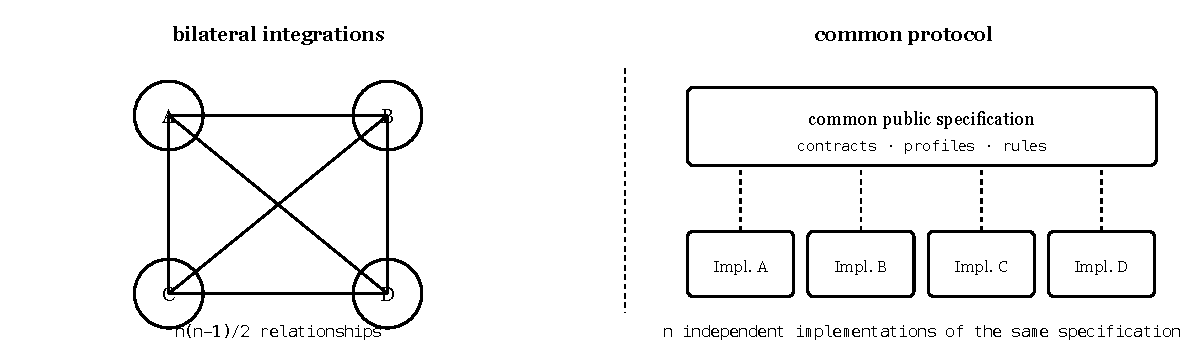
\includegraphics[
    width=0.9\linewidth,
    trim={0cm 0.06cm 0cm 0.06cm},
    clip
  ]{figures/fig1-bilateral-vs-protocol.en.pdf}
  \caption{Complete bilateral mesh and common protocol. In the second regime the shared element is the public specification, not a central infrastructure.}
  \label{fig:bilateral}
\end{figure}

A common protocol does not imply a common infrastructure. In the BANZA model each operator keeps its own implementation, infrastructure and operational relationships, provided it observes the specified behaviour and publishes the artifacts required by the version and profile it adopts: no central BANZA infrastructure is traversed by messages, funds or decisions. Interoperability can also be provided by shared and centralised infrastructures, which continue to perform routing, clearing, settlement or other operational functions. BANZA does not seek to replace them: it adds an open layer of specifications, profiles, public and versioned contracts, deterministic conformance and verifiable evidence, with which an implementation can coexist with different infrastructures, switching systems, schemes or networks.

Standards such as ISO 20022 [1], ISO 8583 [2], the EMV specifications for QR payments [3] and ISO/IEC 9646 [4] address components of messaging, payments and conformance testing. Mojaloop [9] sits closer to BANZA: it combines an interoperability specification between providers --- which admits either direct connection between them or connection mediated by a switch --- with an open-source platform whose operational architecture of central services is used to run schemes, together with its own integration-testing instrumentation. Both specify aspects of the same payment-interoperability space and differ chiefly in how they organise the authority of the specification, the implementation, the conformance evidence and the operational scheme. BANZA complements these works by defining an open protocol in which each implementation publishes artifacts at its canonical origin, is evaluated against a public version and profile, and produces results bound to the inputs observed --- about implementations, not about entities.

This document is descriptive and non-normative: the requirements are defined by the versioned artifacts that the BANZA Normative Manifest identifies. The reference implementation realises the protocol without defining it; the architecture decision records document rationale and are not implementation authority; and the BanzAI explains and makes the public surface navigable without determining conformance. What follows is the model and the architecture (Sections \ref{sec:model} and \ref{sec:architecture}), the profiles (\ref{sec:profiles}), discovery, identity and trust (\ref{sec:discovery}), validation and evidence (\ref{sec:validation}, \ref{sec:evidence}), security and governance (\ref{sec:security}, \ref{sec:governance}), limitations and state (\ref{sec:limitations}, \ref{sec:state}), and the conclusions (\ref{sec:conclusion}).


\section{Model}\label{sec:model}

BANZA distinguishes an operator --- the responsible entity --- from an implementation, the technical system being evaluated. One operator may publish several, and any result always applies to a determinate implementation, version, profile, environment, scope, evidence set and validity period, never to an entity in the abstract.

Each implementation has a stable identifier, and the exact set of artifacts evaluated is fixed by a content digest: a different build is a distinct evaluation subject and requires its own evaluation.

We model an implementation as a six-element tuple. In Equation \eqref{eq:tuple}, \(o\) identifies the operator, \(i\) the implementation, \(v\) the protocol version, \(p\) the conformance profile, \(e\) the environment and \(u\) the canonical origin.

\begin{equation}
\mathcal{I} = (o,\, i,\, v,\, p,\, e,\, u)
\tag{2}\label{eq:tuple}
\end{equation}

The language, the database, the infrastructure provider and the origin of the code are not part of this tuple: conformance depends on the contracts and on observable behaviour, not on internal technology nor on use of the reference implementation.

The artifacts observed at the origin at an instant \(t\) form the set of Equation \eqref{eq:artifacts}, where \(n\) is the number of artifacts.

\begin{equation}
A_t(\mathcal{I}) = \{\, a_1,\, a_2,\, \dots,\, a_n \,\}
\tag{3}\label{eq:artifacts}
\end{equation}

The normative surface of each version is not implicit: it is identified by the \emph{BANZA Normative Manifest}, a versioned index declaring which artifacts define requirements and which do not. Determining what must be implemented is therefore a lookup in published material, not an inference from the code.

Validation takes those artifacts and the specification \(S\) applicable to version \(v\) and profile \(p\); engine version \(m\) produces the result \(R\) --- verdict and reason code ---, the evidence \(E\) and the receipts \(P\).

\begin{equation}
V_m\!\left(A_t(\mathcal{I}),\, S_{v,p}\right) \rightarrow (R,\, E,\, P)
\tag{4}\label{eq:validation}
\end{equation}

Scope is explicit: a result declares the profile, the version, the environment and the evidence consumed, holds only for that combination, and is not extrapolated to the entity that published the artifact. Reproducibility is central: given equivalent canonical inputs, the same specification, profile and engine version, independent executions produce semantically equivalent verdicts and reason codes. The motivation is that of reproducible research [8], but the equivalence is not an analogy --- the protocol defines it normatively, requiring equality of the decisional statuses, of the bindings to the observed inputs and of the set of core reason codes. Non-deterministic metadata is excluded by definition, and byte equality is neither required nor used as the criterion.

\begin{figure}[H]
  \centering
  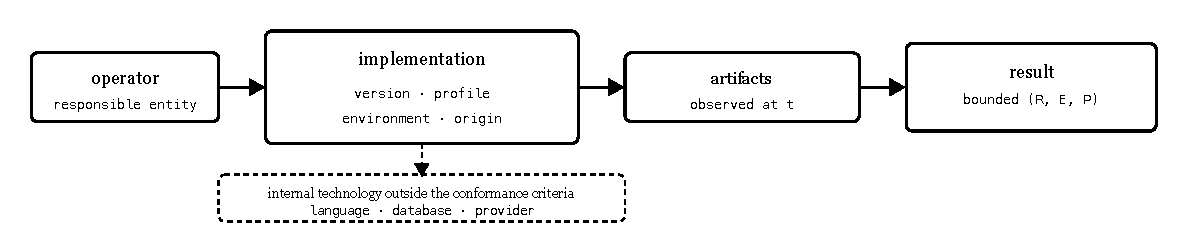
\includegraphics[width=0.9\linewidth, trim={0cm 0.06cm 0cm 0.06cm}, clip]{figures/fig2-model.en.pdf}
  \caption{The result is bounded by the implementation and by the artifacts observed; internal technology is not part of the conformance criteria.}\label{fig:model}
\end{figure}

Content digests, computed with SHA-256 [5], identify and compare exactly the inputs observed. Together with the availability of those inputs, they turn a validation claim into a technical basis that can be re-evaluated by third parties.

Comparing digests requires equivalent representations to produce the same bytes. For JSON artifacts that are signed or digested, BANZA defines \emph{BANZA Canonical JSON} (BCJ/1), a restricted profile of the JSON Canonicalization Scheme [10]: a deterministic UTF-8 representation, rejection of duplicate members rather than their resolution, integers restricted to the interoperable safe domain, and no verifier-side Unicode normalization. Duplicate rejection precedes semantic interpretation, because a parser that applies the first or the last occurrence has already lost the distinction the signature was meant to cover. The numeric domains of this version were audited and no field requires integer representation above the profile's domain.


\section{Architecture}\label{sec:architecture}

BANZA is organised in three institutional layers, separated by responsibility, infrastructure and keys. Layer 1 --- Open protocol brings together specifications, contracts, profiles and common mechanisms for discovery, identity, trust, revocation and federation. Layer 2 --- Conformance and Interoperability Certification evaluates implementations against public profiles and versions, with deterministic engines and verifiable evidence. Layer 3 --- Independent operational schemes comprises infrastructures, networks and schemes that may adopt BANZA and remain subject to their own legal, commercial and regulatory rules.

The architecture rests on five architectural invariants: \emph{open specification} --- the applicable rules, contracts and profiles are public and versioned; \emph{implementation independence} --- no particular implementation constitutes the protocol, and the reference implementation realises it without defining it; \emph{independent verification} --- the published artifacts must suffice for a third party to assess the applicable conditions without depending on a private decision; \emph{operational independence} --- no central infrastructure is required to carry messages or funds; and \emph{separation of decisions} --- conformance evaluation, technical certification, admission to a scheme, operational agreements and regulatory authorisation are distinct processes.

\begin{figure}[H]
  \centering
  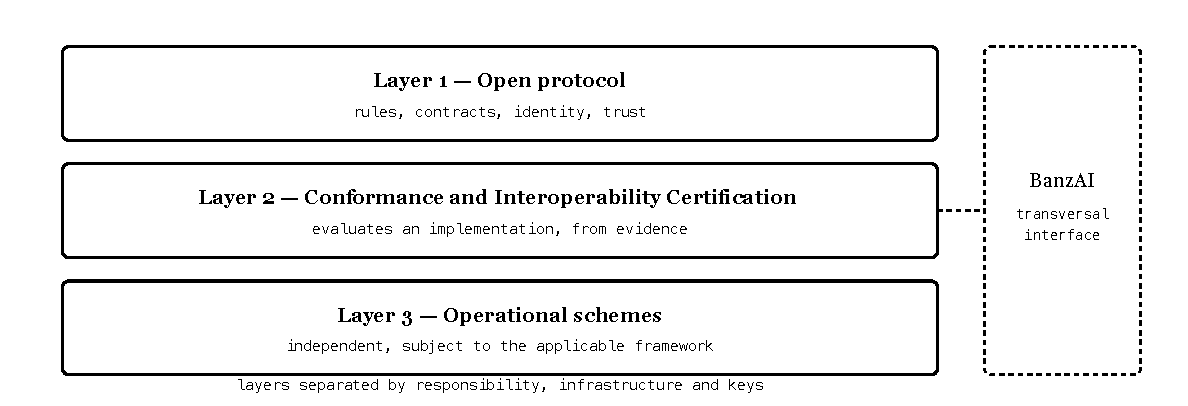
\includegraphics[width=0.9\linewidth, trim={0cm 0.06cm 0cm 0.06cm}, clip]{figures/fig3-three-layers.en.pdf}
  \caption{Layer 1 defines the specification, Layer 2 evaluates conformance through evidence, and Layer 3 remains operationally independent. The BanzAI is transversal, not a fourth layer.}
  \label{fig:layers}
\end{figure}

Technical adoption consists of implementing the public specification and satisfying the applicable contracts: it requires neither the reference implementation's code, nor a connection to a central service, nor prior authorisation. Demonstrating conformance, obtaining certification, joining a scheme and operating in a market are distinct acts. The BanzAI is a human-facing interface for consultation and explanation, without taking part in the technical determination. The L0--L4 profiles of Section \ref{sec:profiles} are distinct from the three layers.

\section{Profiles}\label{sec:profiles}

BANZA defines five cumulative levels, from L0 to L4. Adoption proceeds through the choice of a profile, the publication of artifacts at the canonical origin and the validation journey. A positive result is evidence that the technical conditions of the level are satisfied; it is not certification, authorisation or admission.

L0 --- Protocol Sandbox validates safe configuration in a test environment, with a valid manifest and correct monetary representation. L1 --- Core Payment Capability adds essential payment and traceability capabilities. L2 --- Payment Initiation Capability adds initiation by request or dynamic QR code. L3 --- Inter-Operator Interoperability adds requirements and evidence of interoperability between operators, including technical conditions of routing, settlement and reconciliation --- functions that continue to be performed by the applicable operators or schemes --- and constitutes the federation threshold, requiring evidence involving more than one operator.

The capabilities each profile requires are identified by a common normative vocabulary, and satisfaction is decided by exact comparison of the published identifiers, without implicit normalization. The public vectors likewise have a scope determined by the profile: the association between case and level is declared, not inferred.

L4 --- External Interoperability inherits L3 in full and adds no universal normative artifacts of its own: its requirements and evidence come from an external-interoperability profile identified by identifier and version, and the demonstration is confined to that profile. Satisfying L3 therefore does not satisfy L4 --- with no profile selected the level remains unevaluated, not approved --- and as of this edition no concrete external profile is published.

Levels L0 to L2 can be assessed within a single operator. A certification profile is distinct: it fixes a level and the capabilities, contracts and endpoints required.

\begin{figure}[H]
  \centering
  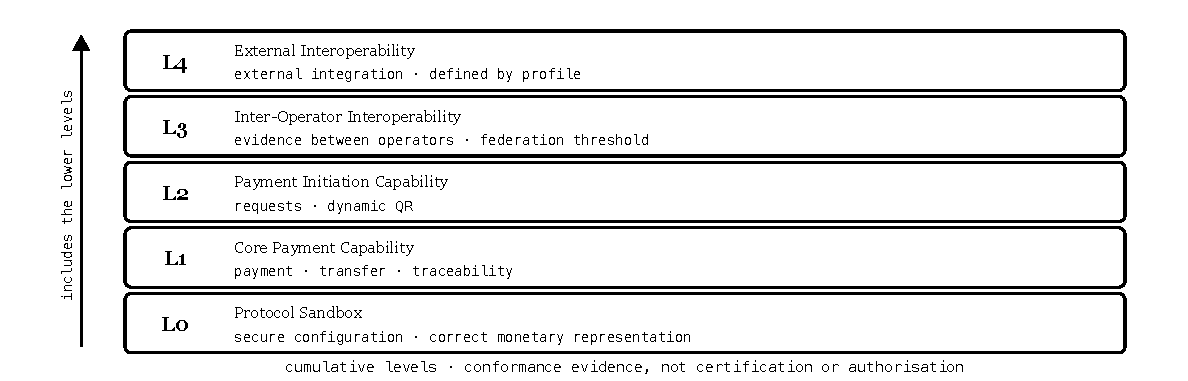
\includegraphics[width=0.9\linewidth,trim={0cm 0.06cm 0cm 0.06cm},clip]{figures/fig4-profiles.en.pdf}
  \caption{The profiles are cumulative. L3 adds evidence between operators and the technical federation threshold. L4 inherits L3 and adds no universal artifacts of its own: its requirements and evidence come from the selected external-interoperability profile, so satisfying L3 does not satisfy L4.}\label{fig:profiles}
\end{figure}


\section{Discovery}\label{sec:discovery}

Each implementation publishes its artifacts at a canonical origin controlled by the operator [7]. Discovery begins at a fixed path under that origin and returns what is needed to identify the implementation, the version, the profile, the endpoints, the signed metadata and the public keys. The Technical Registry may index them, but its presence is not approval and does not replace evaluation.

\begin{figure}[H]
  \centering
  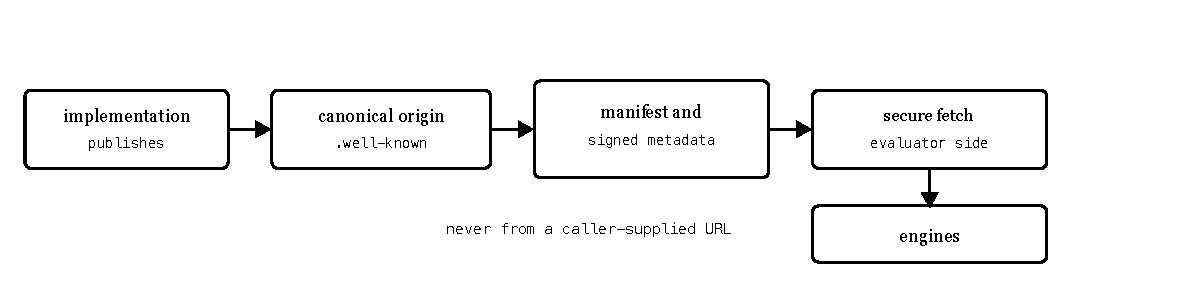
\includegraphics[width=0.9\linewidth,trim={0cm 0.06cm 0cm 0.06cm},clip]{figures/fig5-discovery.en.pdf}
  \caption{The implementation publishes at its canonical origin; the evaluator obtains the artifacts through a secure-fetch module. Discovery depends on no private decision.}\label{fig:discovery}
\end{figure}

Identity and integrity rest on published keys and signed metadata. A trust root, kept offline, signs only the Key Manifest with Ed25519 [6]; that manifest authorises delegated keys separated by domain, which sign the corresponding artifacts. Revocation and validity control reject revoked or expired material.

Trust material is versioned, and validity alone does not distinguish the current version from an earlier one still inside its period. The verifier therefore retains state about what it has already observed: once material is accepted at an ordering point, a later regression is rejected; re-presentation of the same point with the same signing input is an idempotent observation; different content at the same point is a local conflict and is likewise rejected, so that the outcome does not depend on the order of retrieval. The property is local to each verifier's state: it constitutes neither global transparency nor consistency across observers.

The secure-fetch module resolves the target from the canonical origin and applies the security constraints defined by the protocol.


\section{Validation}\label{sec:validation}

Validation follows a fixed journey of eight technical steps and one aggregation step, executed by deterministic engines, each with one of four statuses: verified, pending, failed or blocked. Evaluation is fail-closed --- absent, expired or inconsistent evidence never produces approval --- and certification readiness requires every step of the profile verified, without constituting certification.

The separation between determination and explanation also exists within the result: the status determines the technical outcome, the reason code explains it. A conformant consumer derives its behaviour from the status and never changes a verdict because of a code, which allows the explanatory vocabulary to be extended without changing decisions; and because statuses and codes are public, independent implementations reach semantically equivalent results over the same inputs. The BanzAI presents and explains, without altering. Technical certification is a distinct process that binds an implementation to a public versioned profile.

The required behaviour is verifiable from published material: the contracts define inputs, outputs and observable statuses, and the public vectors fix cases with an expected outcome. For operations to which idempotency applies, the specification defines the key scope, what makes two requests the same request, conflicting reuse and the minimum retention --- observable operational behaviour, not merely evaluation criteria.

\begin{figure}[H]
  \centering
  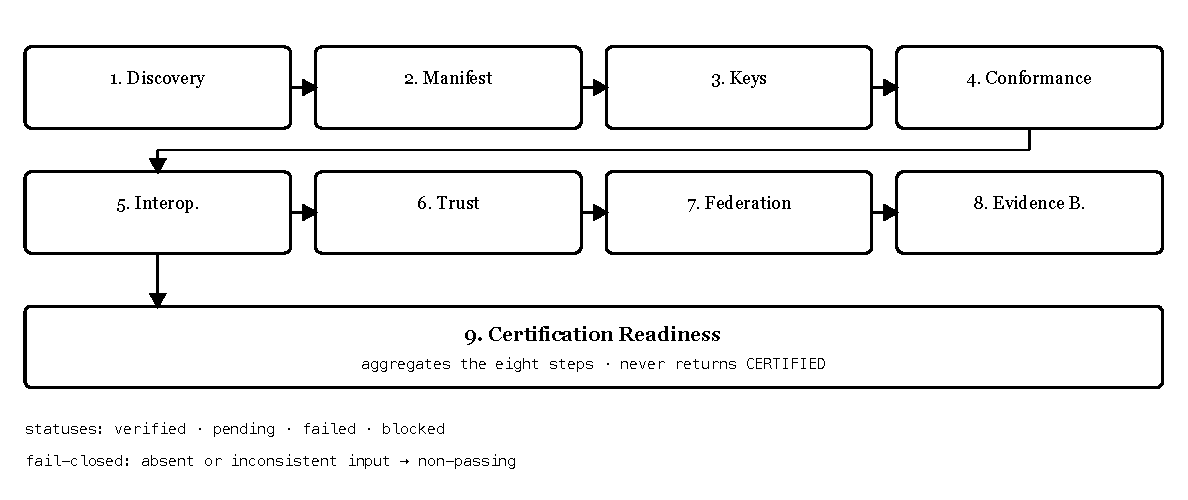
\includegraphics[width=0.9\linewidth,trim={0cm 0.06cm 0cm 0.06cm},clip]{figures/fig6-journey.en.pdf}
  \caption{Eight technical steps and one aggregation step. Certification readiness aggregates the steps required by the applicable profile and does not constitute certification.}
  \label{fig:journey}
\end{figure}

Figure \ref{fig:example} shows the directional evaluation of an implementation B by an evaluator A: B publishes its material, A obtains the artifacts from the canonical origin and evaluates locally. BANZA provides the verifiable technical basis; the operational use of the result remains under A's policy.

\begin{figure}[H]
  \centering
  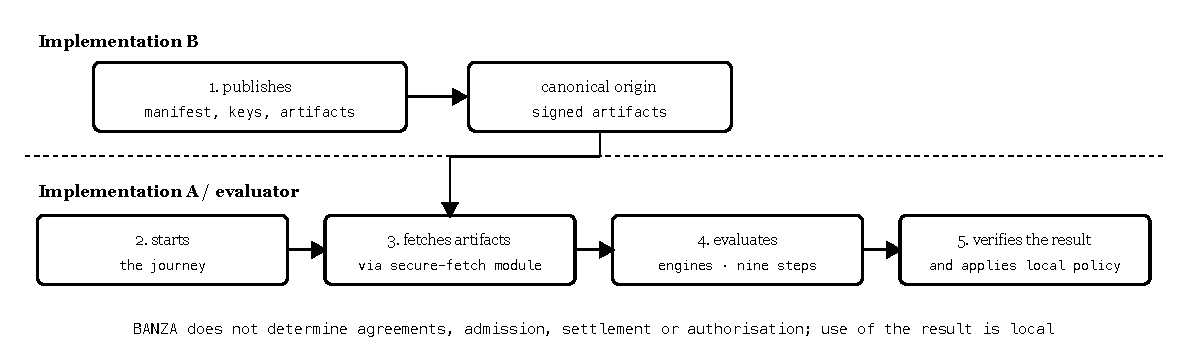
\includegraphics[width=0.9\linewidth,trim={0cm 0.06cm 0cm 0.06cm},clip]{figures/fig7-example.en.pdf}
  \caption{A\(\rightarrow\)B evaluation: B publishes verifiable material, A evaluates locally and can reproduce the result. No central intermediary between A and B.}
  \label{fig:example}
\end{figure}


\section{Evidence}\label{sec:evidence}

Each validation produces results, receipts and verifiable evidence. The receipts record the steps and bind each result to the version, the profile, the artifacts consumed, their digests and the reason codes, allowing the technical basis of the evaluation to be confirmed or reproduced.

\begin{figure}[H]
  \centering
  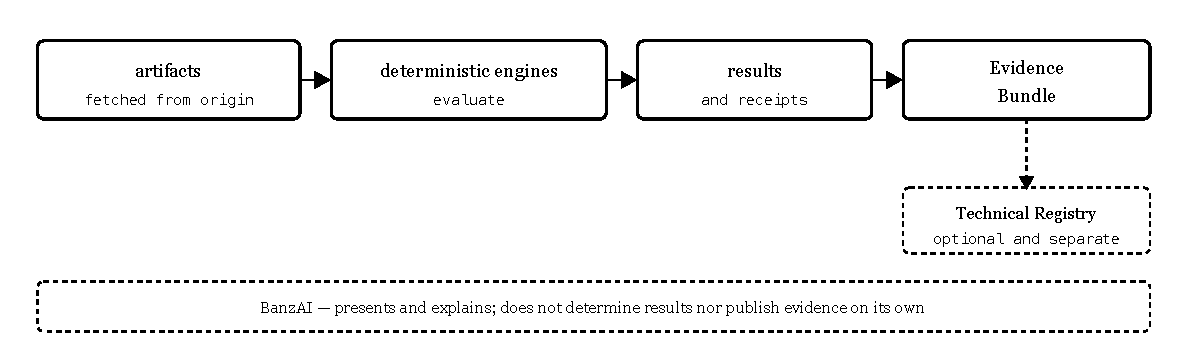
\includegraphics[width=0.9\linewidth,trim={0cm 0.06cm 0cm 0.06cm},clip]{figures/fig8-evidence.en.pdf}
  \caption{The engines evaluate artifacts and produce results and receipts; the Evidence Bundle gathers verifiable material. Publication in the Technical Registry is optional.}
  \label{fig:evidence}
\end{figure}

A receipt represents the state observed at the instant of evaluation; later changes require a new evaluation. The Evidence Bundle gathers the artifacts and references that support the result, without constituting certification or conferring operational status. The absence of an entry in the Technical Registry is not a prohibition and its presence is not an authorisation. Independent verification requires the evidence to suffice for a third party to repeat the applicable steps without depending on any private decision.


\section{Security}\label{sec:security}

The threat model pairs each threat with a determinate mechanism: artifact tampering is detected by signatures and digests; an invalid origin is excluded by resolution from the canonical origin and by secure-fetch validation; revoked or expired material is rejected; challenge replay is prevented by single-use challenges; SSRF and DNS rebinding are blocked by hardened remote fetching; absent or inconsistent evidence leads to fail-closed evaluation; and monotonic observation protects against regression and against conflicting content at the same ordering point, within the limits already stated. None of these mechanisms depends on implicit trust in the origin or in the operator being evaluated.

These properties are distinct and do not substitute for one another: the signature establishes authenticity; validity and revocation, whether the material is usable now; the monotonic state prevents old material, correctly signed and still valid, from replacing more recent material already observed, and detects distinct content at the same ordering point. None provides a verifiable public history or consistency across observers, and on a first observation staleness is not detectable.

The secure-fetch module is the only component that reaches the operator's endpoints. The target is resolved from the canonical origin, never from an arbitrary URL supplied by the caller; the module accepts only HTTPS, blocks private, local and cloud-metadata addresses, connects only to previously validated addresses, follows no redirects, validates TLS and bounds responses. These are observable requirements, independent of any internal technology.


\section{Governance}\label{sec:governance}

BANZA evolves through public and versioned instruments: RFCs structure proposals, ADRs record architecture decisions. Versioning is explicit --- incompatible changes require a new major version, compatible ones enter minor or patch versions. Each implementation declares the version and profile it adopts, and a certification profile is immutable once published.

The openness of the protocol does not eliminate governance, but governance determines how the rules evolve without making the protocol maintainer a technical intermediary between implementations. Implementing a published version is distinct from having authority to change it: conformance requires satisfying the applicable contracts, whereas changing the rules follows the public decision and versioning process.

\begin{figure}[H]
  \centering
  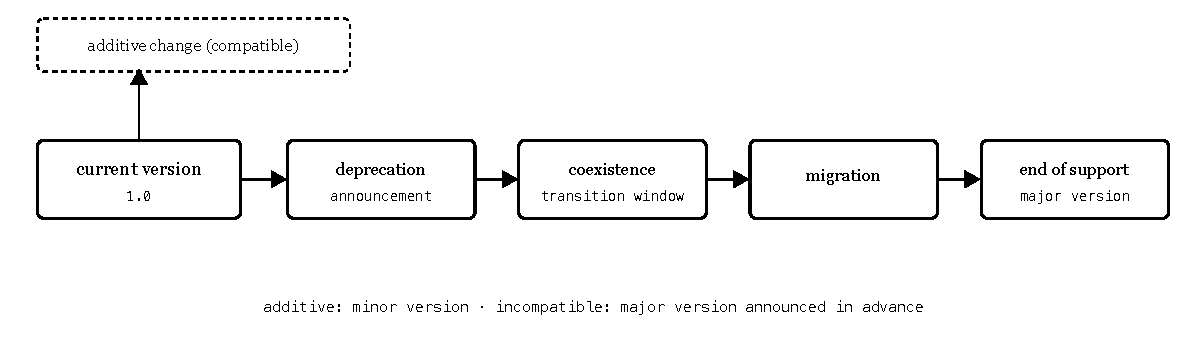
\includegraphics[width=0.9\linewidth,trim={0cm 0.06cm 0cm 0.06cm},clip]{figures/fig10-governance.en.pdf}
  \caption{Protocol evolution separates proposal, recorded decision and versioned publication. Governing rules is not operating transactions nor authorising participants.}
  \label{fig:governance}
\end{figure}

Incompatible changes are announced with a migration path, allowing temporary coexistence; deprecation is explicit and phased. The current version of the protocol is 1.0.0.

\section{Limitations}\label{sec:limitations}

BANZA's guarantees have clear boundaries. They are technical, not regulatory: a positive result demonstrates conformance with a public profile, without implying authorisation to operate, admission to a scheme or a commercial agreement.

Second, they apply to what is observed: reproducibility covers deterministic evaluations over the declared inputs, not the operator's internal controls nor behaviour outside the protocol, and a compromised origin or key is detectable only when the compromise manifests in observable signals or in revocation material.

Third, the openness of the specification does not by itself demonstrate the ease of independent implementation: that property depends on the completeness of the contracts, the quality of the vectors and the ability of an external team to build a conformant implementation without recourse to the reference code. Likewise, the integration with external infrastructures envisaged by the architecture does not demonstrate effective access to those infrastructures, which may depend on interfaces, agreements, scheme rules or authorisation.

Fourth, some boundaries follow from the current design: trust material is published at a single canonical point, without replicas, and fail-closed evaluation preserves the correctness of the decision while unavailable fresh material may prevent a new evaluation; the monotonic state of Section \ref{sec:discovery} is local to each verifier and does not establish consistency across observers; and with no concrete external profile published, L4 has not yet been demonstrated. Finally, the evidence presented here is architectural: it demonstrates mechanisms in the reference implementation and does not measure performance, scale or adoption. A package completeness rehearsal verified that the public package for profile L0 is sufficient and closed upon itself, which does not demonstrate that an external team can implement from it, and interoperability in production between unrelated organisations is not demonstrated.


\section{State}\label{sec:state}

BANZA remains in pre-production: the Technical Registry contains zero production operators and zero active technical certifications, payments with real money are disabled and the empty registry is the expected state. The reference implementation, Operator Zero, runs in an isolated test environment with demonstration currency, moves no real funds, remains uncertified and is evaluated by the same contracts and the same journey as any other implementation.

The normative surface is explicitly indexed, and the set required by each profile derives from that indexing. From it a public distribution was prepared for profile L0, without the reference implementation's code; a package completeness rehearsal verified that the material is closed upon itself, resolving all references internally, with no requirement dependent on the source repository, the decision records or the BanzAI, and identified real questions, since corrected.

The completeness of a distribution and the capability for independent implementation are distinct properties: the first was verified, the second was not, and it remains to be demonstrated through a third-party implementation built without recourse to the reference code.

Demonstrating it convincingly will require an external implementation built from the public specifications and contracts, without recourse to the reference code, able to satisfy the applicable conformance vectors and to take part in a directional evaluation with another implementation, producing semantically equivalent results and verifiable evidence. The success of such a trial would demonstrate independent implementation capability, and would still not amount to regulatory authorisation, admission to a scheme or use in production.


\section{Conclusions}\label{sec:conclusion}

This work presented BANZA as an open financial interoperability protocol whose definition does not depend on any particular implementation and whose conformance is assessed through deterministic mechanisms and verifiable evidence, without mandatory central infrastructure for messages or funds.

The main contributions are:

\begin{itemize}
  \item evaluation of implementations against public versions and profiles rather than of entities in the abstract, with conformance depending on observable behaviour and not on the origin of the code;

  \item separation between protocol, certification and operational schemes, keeping technical conformance, admission, operational agreements and regulatory authorisation distinct;

  \item a public, versioned and explicitly indexed normative surface, with a deterministic canonical representation for signed or digested artifacts;

  \item public execution semantics --- statuses, reason codes, idempotency --- and conformance vectors with a scope declared per profile;

  \item deterministic validation bound to the inputs through digests, receipts and verifiable evidence, with cumulative profiles and fail-closed evaluation;

  \item separation between technical determination, operational decision and explanation assisted by the BanzAI.
\end{itemize}

These contributions rest on the five architectural invariants stated in Section \ref{sec:architecture} --- open specification, implementation independence, independent verification, operational independence and separation of decisions --- which remain the criteria by which the protocol should be assessed.

These properties define an architectural direction, not a maturity already attained: the boundaries stated in Section \ref{sec:limitations} remain to be lifted. Future work should test implementation independence directly through distinct teams, assess the resulting interoperability and measure reproducibility across evaluators, performance, scalability, integration costs and the application of external-interoperability profiles.

In summary, BANZA makes the technical basis of interoperability public and verifiable without becoming a mandatory operational intermediary: different implementations adopt the same specification, demonstrate that they satisfy the applicable requirements and produce evidence that third parties can reproduce.


% Manual reference list with explicit [1]--[10] labels (engine-independent; avoids the copernicus natbib
% author-year mode, which does not print numeric \bibitem labels). The body cites the literal [1]--[10].
\newpage
\section*{\refname}
{\small
\begin{list}{}{%
  \setlength{\labelsep}{0.5em}%
  \setlength{\labelwidth}{1.8em}%
  \setlength{\leftmargin}{2.3em}%
  \setlength{\itemindent}{0pt}%
  \setlength{\itemsep}{3pt}%
  \setlength{\parsep}{0pt}}
\sloppy
\item[{[1]}] International Organization for Standardization. ISO 20022 --- Financial services --- Universal financial industry message scheme. ISO. https://www.iso20022.org/
\item[{[2]}] International Organization for Standardization. ISO 8583:2023 --- Financial-transaction-card-originated messages --- Interchange message specifications. Edition 3. ISO, 2023. https://www.iso.org/standard/79451.html
\item[{[3]}] EMVCo, LLC. EMV QR Code Specification for Payment Systems (EMV QRCPS): Merchant-Presented Mode, Version 1.1. EMVCo, November 2020. https://www.emvco.com/
\item[{[4]}] International Organization for Standardization / International Electrotechnical Commission. ISO/IEC 9646-1:1994 --- Information technology --- Open Systems Interconnection --- Conformance testing methodology and framework --- Part 1: General concepts. ISO/IEC, 1994.
\item[{[5]}] National Institute of Standards and Technology (NIST). Secure Hash Standard (SHS). FIPS PUB 180-4. NIST, August 2015. DOI 10.6028/NIST.FIPS.180-4. https://nvlpubs.nist.gov/nistpubs/fips/nist.fips.180-4.pdf
\item[{[6]}] S. Josefsson and I. Liusvaara. Edwards-Curve Digital Signature Algorithm (EdDSA). RFC 8032, IRTF, January 2017. DOI 10.17487/RFC8032. https://www.rfc-editor.org/rfc/rfc8032
\item[{[7]}] M. Nottingham. Well-Known Uniform Resource Identifiers (URIs). RFC 8615, IETF, May 2019. DOI 10.17487/RFC8615. https://www.rfc-editor.org/rfc/rfc8615
\item[{[8]}] R. Peng. Reproducible Research in Computational Science. Science, 334(6060):1226--1227, 2011. DOI 10.1126/science.1213847. https://doi.org/10.1126/science.1213847
\item[{[9]}] Mojaloop Foundation. Open API for FSP Interoperability (FSPIOP) Specification and Mojaloop open-source platform. https://docs.mojaloop.io/
\item[{[10]}] A. Rundgren, B. Jordan and S. Erdtman. JSON Canonicalization Scheme (JCS). RFC 8785, IETF, June 2020. DOI 10.17487/RFC8785. https://www.rfc-editor.org/rfc/rfc8785
\end{list}}

\end{document}
